\documentclass[11pt]{article}

% Switch to "final" for camera-ready, "preprint" for non-anonymous arXiv.
\usepackage[review]{acl}

% ---- Standard ACL preamble ----
\usepackage{times}
\usepackage{latexsym}
\usepackage[T1]{fontenc}
\usepackage[utf8]{inputenc}
\usepackage{microtype}
\usepackage{graphicx}

% ---- Math / tables / graphics extras used in this paper ----
\usepackage{amsmath}
\usepackage{amssymb}
\usepackage{booktabs}
\usepackage{multirow}
\usepackage{xcolor}
\usepackage{subcaption}
\usepackage{tikz}
\usetikzlibrary{positioning,arrows.meta,calc,fit,backgrounds,shapes.geometric}

\usepackage{url}

% ---- Convenient macros ----
\newcommand{\methodname}{InfoGate}
\newcommand{\Lvtask}{\mathcal{L}_{\text{task}}}
\newcommand{\Lvtib}{\mathcal{L}_{\text{tib}}}
\newcommand{\Lvlib}{\mathcal{L}_{\text{lib}}}
\newcommand{\Lvrib}{\mathcal{L}_{\text{rib}}}
\newcommand{\KL}{\mathrm{KL}}
\newcommand{\softmax}{\mathrm{softmax}}
\newcommand{\sigmoid}{\sigma}
\newcommand{\conf}{\mathbf{c}}
\newcommand{\bn}{\mathbf{B}}
\newcommand{\matr}[1]{\mathbf{#1}}

\title{\methodname: Information-Bottleneck-Guided Adaptive\\
       Cross-Attention for Multimodal Sentiment Analysis}

\author{Anonymous EMNLP submission \\
  \texttt{infogate.author@example.org} \\
}

\begin{document}
\maketitle

\begin{abstract}
Multimodal Sentiment Analysis (MSA) integrates language, acoustic and visual signals to estimate utterance-level sentiment intensity. State-of-the-art systems combine cross-modal attention with information-bottleneck (IB) compression, but they (i)~weight every auxiliary token equally, regardless of how informative it is, (ii)~inject auxiliary cues with a fixed strength even when the auxiliary signal contradicts the primary modality, and (iii)~commit to a single language-centric primary modality before observing the sample. We present \methodname, a framework that uses a single signal -- the per-token confidence $\sigmoid(-\log \sigma^{2})$ extracted from a variational IB encoder -- to modulate three different stages of multimodal fusion: token-level attention reweighting, sample-level alignment-modulated injection, and global per-sample primary-modality routing. \methodname{} is trained end-to-end with a task loss, token- and label-IB losses, and a stage-2 routing-IB loss that supervises the modality selector with per-modality task error. With Bayesian hyper-parameter search on three benchmarks, \methodname{} reaches state-of-the-art MAE on \textsc{CMU-MOSI} ($0.5923$), \textsc{CMU-MOSEI} ($0.4941$) and \textsc{CH-SIMS}~v2 ($0.3138$), while also offering a competing trade-off with $88.85\%$ Acc-2 / $88.83\%$ F1 on \textsc{CMU-MOSI}.

\end{abstract}

\section{Introduction}
\label{sec:intro}
Multimodal Sentiment Analysis
\citep{zadeh2016mosi,zadeh2018mosei,liu2022simsv2}
predicts the sentiment intensity of an utterance from three loosely
aligned streams: language, acoustic prosody and facial dynamics.
The dominant design pattern is to use a strong text encoder
(BERT-style) as the primary backbone and inject acoustic / visual
context through cross-modal attention or low-rank fusion
\citep{rahman2020magbert,tsai2019mult,yu2021selfmm,han2021mmim}.
Recent work adds an information-bottleneck (IB) regulariser to compress
each modality into a task-relevant subspace
\citep{ithp2024,wu2023dbf,cmib2023,camib2026}, which improves the
state-of-the-art MAE on \textsc{CMU-MOSI} and \textsc{CMU-MOSEI}.

Three weaknesses persist across this line of work:
\textbf{(W1)} Cross-modal attention treats every auxiliary token as
equally informative.
A whispered \textit{``yeah''} and a screamed \textit{``yeah''} have
identical text content but very different acoustic information; current
key/value gating does not see this distinction.
\textbf{(W2)} The injection strength of auxiliary tokens into the
primary stream is fixed regardless of \emph{cross-modal consistency}.
A smiling face during a sarcastic verbal utterance contradicts the
language signal, but is added to the primary representation with the
same weight as a corroborating face.
\textbf{(W3)} Most architectures pre-commit to a fixed primary
modality, usually text.
Recent dynamic-routing approaches such as MODS \citep{wang2023cross}
introduce a learned modality selector, but the selector is trained from
the task gradient alone and tends to collapse onto the easy text-only
prior.

We argue that all three weaknesses share a single root cause: the
absence of a calibrated, sample-wise notion of \emph{information
quality} that can be propagated through the fusion pipeline.
We provide one.
The variational IB encoder used by ITHP and CyIN already produces a
per-token log-variance $\log\sigma^{2,m}$, and we observe that the
corresponding confidence
$\conf^{m}=\sigmoid(-\log\sigma^{2,m})$
is a natural, end-to-end-learnable measure of how task-relevant a token
is.
We use it once to modulate \emph{everything} downstream.

Concretely, our model \methodname{} (Figure~\ref{fig:overview}) uses
$\conf^{m}$ at three different scales:
\begin{itemize}
\itemsep0.1em
\item \textbf{Token level} -- IB-Guided Cross-Attention biases scores
  by $\gamma\log\bar c^{a}$ and gates values by $\bar c^{a}$, so noisy
  auxiliary positions are simultaneously down-weighted in attention and
  in contribution (\S\ref{sec:method:ibca}).
\item \textbf{Sample level} -- Alignment-Modulated Injection scales
  each cross-attention output by the cosine similarity of the primary
  and auxiliary bottleneck representations, lower-bounded at $0.3$;
  the injection therefore contracts when modalities disagree
  (\S\ref{sec:method:align}).
\item \textbf{Global level} -- a Gumbel-softmax modality selector
  picks one of the three modalities as the primary stream per sample,
  supervised in stage 2 by a routing-IB loss whose teacher signal is
  the per-modality task error in the bottleneck space
  (\S\ref{sec:method:mselector}).
\end{itemize}
This single mechanism resolves \textbf{W1--W3} simultaneously and is
fully differentiable through a single $\log\sigma^{2}$ pathway.

Our contributions are: (i)~the \emph{IB-confidence-as-modulation}
principle that unifies token, sample and global filtering through one
back-propagatable signal; (ii)~the IB-Guided Cross-Attention
mechanism with score bias and value gate; (iii)~the
Alignment-Modulated Injection rule for sample-level cross-modal
consistency control; (iv)~a stage-2 routing-IB loss that supervises
the modality selector with per-modality task error; and
(v)~state-of-the-art results on \textsc{CMU-MOSI} (MAE 0.5923) and
\textsc{CMU-MOSEI} (MAE 0.4941) under careful Optuna search, with a
competitive trade-off on \textsc{CH-SIMS}~v2.
The paper is organised as follows.
\S\ref{sec:related} reviews multimodal sentiment fusion and IB-based
methods.
\S\ref{sec:method} formalises \methodname{}.
\S\ref{sec:exp} reports the main results, ablations and
hyper-parameter search.
\S\ref{sec:analysis} analyses routing behaviour and the
MAE-vs-accuracy trade-off.
\S\ref{sec:conclusion} concludes; limitations and ethics statements
follow.


\section{Related Work}
\label{sec:related}
\paragraph{Multimodal sentiment fusion.}
Early work on \textsc{CMU-MOSI} and \textsc{CMU-MOSEI} aligned
modality-specific recurrent encoders through tensor / outer-product
fusion (TFN \citep{zadeh2017tfn}, LMF \citep{liu2018lmf}, MFN
\citep{zadeh2018mfn}, Graph-MFN \citep{zadeh2018gmfn}).
The transformer era replaced these with cross-modal attention
\citep{tsai2019mult} and BERT-grounded fusion (MAG-BERT
\citep{rahman2020magbert}, MISA \citep{hazarika2020misa}, Self-MM
\citep{yu2021selfmm}, MMIM \citep{han2021mmim}).
A second line of work disentangles modality-shared and
modality-specific subspaces (MFM \citep{tsai2019mfm}, DMD
\citep{li2023dmd}, EMOE \citep{emoe2024}); a third focuses on
cross-modal alignment through contrastive or denoising objectives
\citep{wu2023dbf,boost2024}.

\paragraph{Information bottleneck for multimodal learning.}
The IB principle \citep{tishby2000information,tishby2015dnn} compresses
input $X$ into a bottleneck $B$ by minimising $I(X;B)$ while maximising
$I(B;Y)$.
Its variational form (VIB) \citep{alemi2017vib,kingma2014vae} makes the
objective tractable for deep networks.
ITHP \citep{ithp2024} introduces a hierarchical IB chain for
multimodal perception, while CyIN cyclically translates between
modality bottlenecks; CaMIB \citep{camib2026} adds causal-aware
ingredients to the same recipe.
C-MIB \citep{cmib2023} and DLF \citep{dlf2024} regularise cross-modal
mutual information.
\methodname{} differs from this family in two ways.
First, while existing IB methods use $\log\sigma^{2}$ only inside the
KL term of the VIB objective, we expose it as a \emph{first-class
modulation signal} for downstream attention and gating.
Second, IB methods that perform translation
(CyIN, ITHP) require auxiliary cross-modal decoders even at inference;
\methodname{} does not perform any cross-modal translation and
therefore has a strictly smaller inference-time graph.

\paragraph{Routing and dynamic primary selection.}
MODS \citep{wang2023cross} is the closest predecessor.
It introduces a Modality Selector that uses Gumbel-softmax to pick a
per-sample primary modality, and an equal-weight cross-attention
fusion (PCCA).
\methodname{} reuses the MSelector backbone, but adds the IB-guided
modulation of \S\ref{sec:method:ibca}--\ref{sec:method:gate}, and
supervises the selector in stage 2 with a routing-IB loss that uses
the per-modality task error rather than a fixed text prior.
DEVA \citep{deva2024}, KuDA \citep{kuda2024}, MOAC \citep{moac2025}
and TMSON \citep{tmson2024} are concurrent dynamic-routing or
adaptive-fusion methods compared in Table~\ref{tab:main_mosi_mosei};
none of them couples routing to a per-token IB confidence.
Adaptive Information Gates (Eq.~\ref{eq:adagate}) are also reminiscent
of the gated fusion in MAG-BERT and DBF \citep{wu2023dbf}, but
condition on the IB-compressed bottleneck rather than on raw
features.


\section{Method}
\label{sec:method}
\subsection{Overview}
\label{sec:method:overview}

Let an utterance be represented by three temporally aligned token sequences
$X^{t}\in\mathbb{R}^{T\times d_{t}}$ (text, last hidden states of
DeBERTa-v3-base \citep{he2023debertav3}),
$X^{a}\in\mathbb{R}^{T\times d_{a}}$ (acoustic, COVAREP
\citep{degottex2014covarep}) and
$X^{v}\in\mathbb{R}^{T\times d_{v}}$ (visual, OpenFace 2.0
\citep{baltrusaitis2018openface}).
The goal is to predict a continuous sentiment score $y\in\mathbb{R}$.

\methodname{} is built around a single design principle: the
\emph{IB-derived per-token confidence}
\(\conf=\sigmoid(-\log\sigma^{2})\in[0,1]^{T\times d_{B}}\) is a universal
control signal that can modulate fusion at three different scales
(Figure~\ref{fig:overview}):
\textbf{(i) token level} -- biasing cross-attention scores and gating values
(\S\ref{sec:method:ibca});
\textbf{(ii) sample level} -- modulating the magnitude of cross-modal injection
by the cosine similarity of the bottleneck representations
(\S\ref{sec:method:align});
\textbf{(iii) global level} -- supervising a Gumbel--softmax modality selector
through a stage-2 routing-IB loss (\S\ref{sec:method:mselector}).

\begin{figure*}[t]
\centering
\resizebox{\linewidth}{!}{%
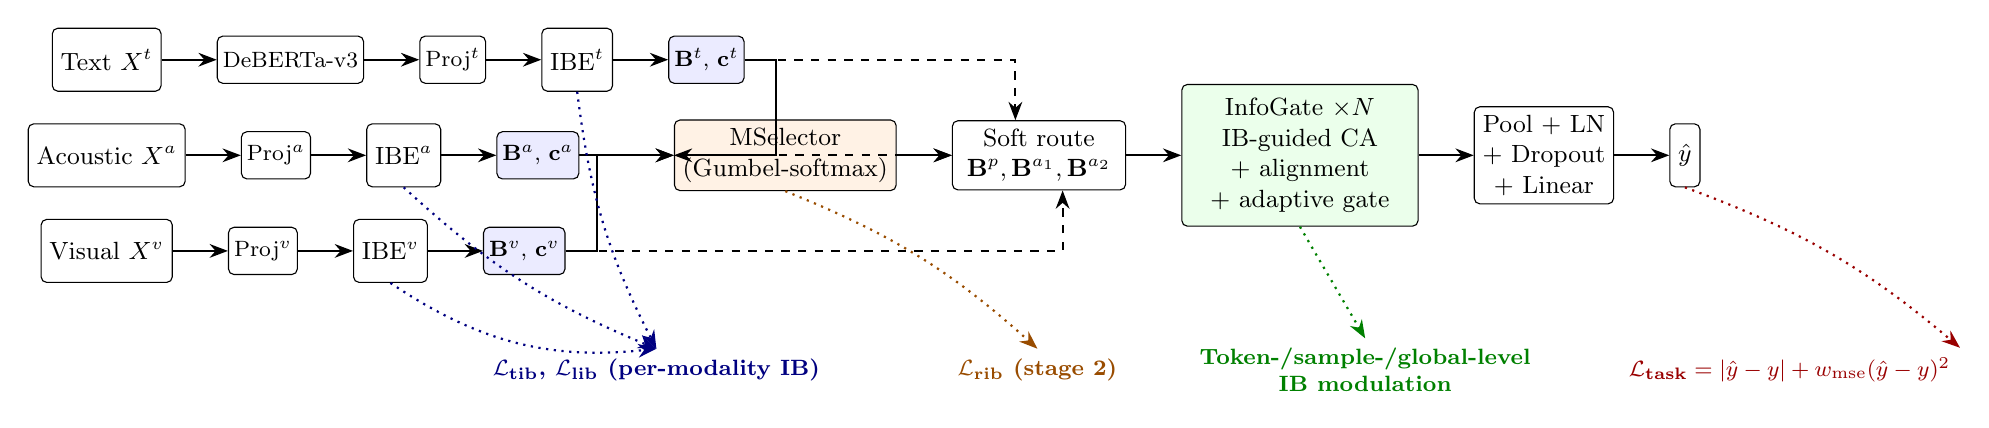
\begin{tikzpicture}[
    node distance=4mm and 7mm,
    every node/.style={font=\small},
    box/.style={draw, rounded corners=2pt, align=center, minimum height=8mm, inner sep=3pt, fill=white},
    smallbox/.style={draw, rounded corners=2pt, align=center, minimum height=6mm, inner sep=2pt, font=\footnotesize, fill=white},
    arrow/.style={-Stealth, thick},
    dashedarrow/.style={-Stealth, thick, dashed},
    confarrow/.style={-Stealth, thick, dotted, draw=black!60},
    grouplabel/.style={font=\bfseries\footnotesize, align=center}
  ]

  % --- Inputs (left) ---
  \node[box] (xt) {Text $X^{t}$};
  \node[box, below=of xt] (xa) {Acoustic $X^{a}$};
  \node[box, below=of xa] (xv) {Visual $X^{v}$};

  % --- DeBERTa for text ---
  \node[smallbox, right=of xt] (dberta) {DeBERTa-v3};

  % --- Projections ---
  \node[smallbox, right=of dberta] (pt) {Proj$^{t}$};
  \node[smallbox, right=of xa] (pa) {Proj$^{a}$};
  \node[smallbox, right=of xv] (pv) {Proj$^{v}$};

  % --- IB encoders ---
  \node[box, right=of pt] (ibt) {IBE$^{t}$};
  \node[box, right=of pa] (iba) {IBE$^{a}$};
  \node[box, right=of pv] (ibv) {IBE$^{v}$};

  % --- Bottleneck + confidence labels ---
  \node[smallbox, right=of ibt, fill=blue!8] (bt) {$\bn^{t},\,\conf^{t}$};
  \node[smallbox, right=of iba, fill=blue!8] (ba) {$\bn^{a},\,\conf^{a}$};
  \node[smallbox, right=of ibv, fill=blue!8] (bv) {$\bn^{v},\,\conf^{v}$};

  % --- MSelector ---
  \node[box, right=12mm of ba, fill=orange!10] (msel) {MSelector\\(Gumbel-softmax)};

  % --- Routing block ---
  \node[box, right=of msel, minimum width=22mm] (route) {Soft route\\$\bn^{p},\bn^{a_{1}},\bn^{a_{2}}$};

  % --- InfoGate stack ---
  \node[box, right=of route, minimum width=30mm, minimum height=18mm, fill=green!8] (ig) {InfoGate $\times N$\\IB-guided CA\\+ alignment\\+ adaptive gate};

  % --- Head ---
  \node[box, right=of ig] (head) {Pool + LN\\+ Dropout\\+ Linear};
  \node[box, right=of head] (yhat) {$\hat{y}$};

  % --- Arrows: inputs to projections ---
  \draw[arrow] (xt) -- (dberta);
  \draw[arrow] (dberta) -- (pt);
  \draw[arrow] (xa) -- (pa);
  \draw[arrow] (xv) -- (pv);

  % --- Projections to IB encoders ---
  \draw[arrow] (pt) -- (ibt);
  \draw[arrow] (pa) -- (iba);
  \draw[arrow] (pv) -- (ibv);

  % --- IB to bottleneck/confidence ---
  \draw[arrow] (ibt) -- (bt);
  \draw[arrow] (iba) -- (ba);
  \draw[arrow] (ibv) -- (bv);

  % --- Bottlenecks into MSelector ---
  \draw[arrow] (bt.east) -- ++(4mm,0) |- (msel.west);
  \draw[arrow] (ba.east) -- (msel.west);
  \draw[arrow] (bv.east) -- ++(4mm,0) |- (msel.west);

  % --- MSelector to route ---
  \draw[arrow] (msel) -- (route);

  % --- Bottlenecks/confidence into route block (data path) ---
  \draw[arrow, dashed] (bt.east) -- ++(2mm,0) -| ([xshift=-3mm]route.north);
  \draw[arrow, dashed] (ba.east) -- ++(2mm,0) -- (route.west);
  \draw[arrow, dashed] (bv.east) -- ++(2mm,0) -| ([xshift=3mm]route.south);

  % --- Routing to InfoGate stack ---
  \draw[arrow] (route) -- (ig);

  % --- InfoGate to head ---
  \draw[arrow] (ig) -- (head);
  \draw[arrow] (head) -- (yhat);

  % --- Loss labels (below) ---
  \node[grouplabel, below=12mm of bv.south west, anchor=west, text=blue!50!black] (libtib) {$\Lvtib$, $\Lvlib$ (per-modality IB)};
  \node[grouplabel, right=15mm of libtib, text=orange!60!black] (lrib) {$\Lvrib$ (stage 2)};
  \node[grouplabel, right=8mm of lrib, text=green!50!black] (lk) {Token-/sample-/global-level\\IB modulation};
  \node[grouplabel, right=10mm of lk, text=red!60!black] (ltask) {$\Lvtask=|\hat y-y|+w_{\mathrm{mse}}(\hat y-y)^{2}$};

  % --- Connection from each IB encoder block (training-only loss) ---
  \draw[confarrow, blue!50!black] (ibt.south) to[bend right=10] (libtib.north);
  \draw[confarrow, blue!50!black] (iba.south) to[bend right=10] (libtib.north);
  \draw[confarrow, blue!50!black] (ibv.south) to[bend right=20] (libtib.north);
  \draw[confarrow, orange!60!black] (msel.south) to[bend left=10] (lrib.north);
  \draw[confarrow, green!50!black] (ig.south) -- (lk.north);
  \draw[confarrow, red!60!black] (yhat.south) to[bend left=10] (ltask.north east);

\end{tikzpicture}%
}
\caption{Overview of \methodname{}. Each modality is projected, encoded by
a variational IB encoder that exposes a per-token confidence
$\conf^{m}=\sigmoid(-\log\sigma^{2,m})$, and routed by a Gumbel-softmax
modality selector. The InfoGate stack (\S\ref{sec:method:ibca}--\ref{sec:method:gate})
uses the same confidence signal at three different scales (token, sample,
global) to modulate cross-attention, alignment-aware injection and
adaptive gating before a primary-only regression head.}
\label{fig:overview}
\end{figure*}


\subsection{Per-Modality Projection and IB Encoder}
\label{sec:method:ib}

Each modality is first projected into a shared $d_{u}$-dimensional space
with $\mathrm{Proj}^{m}(X^{m})$ realised as a linear layer plus ReLU
(text), or LayerNorm-Linear-ReLU (acoustic / visual; the LayerNorm
stabilises the very different feature statistics of the raw COVAREP /
OpenFace streams).
Each projected sequence $F^{m}\in\mathbb{R}^{T\times d_{u}}$ is then fed to
a variational IB encoder $\mathrm{IBE}^{m}$ that returns mean
$\mu^{m}$ and log-variance $\log\sigma^{2,m}$, from which a stochastic
bottleneck representation is sampled with the standard reparameterization
trick \citep{kingma2014vae,alemi2017vib}:
\begin{align}
  (\mu^{m},\log\sigma^{2,m}) &= \mathrm{IBE}^{m}(F^{m}), \\
  \bn^{m} &= \mu^{m} + \boldsymbol{\epsilon}\odot\exp(\tfrac{1}{2}\log\sigma^{2,m}),
\end{align}
with $\boldsymbol{\epsilon}\!\sim\!\mathcal{N}(0,\matr{I})$ during training and
$\bn^{m}=\mu^{m}$ at evaluation.
The IB principle \citep{tishby2000information,tishby2015dnn,alemi2017vib}
encourages the bottleneck to retain only task-relevant information,
making $\log\sigma^{2,m}$ a natural proxy for per-token uncertainty.
We therefore define a per-token, per-dimension \emph{confidence map}
\begin{equation}
  \conf^{m} \;=\; \sigmoid\!\big(-\log\sigma^{2,m}\big)\;\in\;[0,1]^{T\times d_{B}},
  \label{eq:conf}
\end{equation}
which is reused at every later modulation stage.

To make the bottleneck informative we attach an intra-modal decoder
$\mathrm{Dec}^{m}$ for each modality and minimise the
token-level IB objective
\begin{equation}
  \Lvtib \;=\; \sum_{m\in\{t,a,v\}} \KL\big(\mu^{m},\sigma^{2,m}\big) \;+\; \beta_{\mathrm{ib}}\,\mathrm{MSE}\!\big(\mathrm{Dec}^{m}(\bn^{m}),F^{m}\big),
  \label{eq:tib}
\end{equation}
where $\KL(\mu,\sigma^{2}) = -\tfrac{1}{2}\sum_{i}\big(1+\log\sigma_{i}^{2}-\mu_{i}^{2}-\sigma_{i}^{2}\big)$
is the closed-form KL against $\mathcal{N}(0,\matr{I})$, masked over valid
tokens.
A label-level IB term anchors the bottleneck to the sentiment label
through a per-modality linear head $\mathrm{LP}^{m}$:
\begin{equation}
  \Lvlib \;=\; \tfrac{1}{3}\sum_{m}\Big[\KL(\mu^{m}_{\bar{t}},\sigma^{2,m}_{\bar{t}}) + \beta_{\mathrm{ib}}\,|\mathrm{LP}^{m}(\bn^{m}_{\bar{t}})-y|\Big],
  \label{eq:lib}
\end{equation}
where $\bar{t}$ denotes mean-pooling over valid tokens.

\subsection{IB-Guided Cross-Attention}
\label{sec:method:ibca}

Cross-attention from auxiliary modality $a$ to primary modality $p$ is
the standard scaled dot-product mechanism with two confidence-driven
modifications.
For each head, queries are projected from $\bn^{p}$ and keys/values from
$\bn^{a}$ as $Q,K,V$.
Let $\bar{c}^{a}\in\mathbb{R}^{T}$ be the mean of $\conf^{a}$ over the
bottleneck dimension.
We modify the attention as
\begin{align}
  \matr{S} &= \tfrac{1}{\sqrt{d_{h}}}QK^{\top} + \gamma\,\log(\bar{c}^{a}+\varepsilon),
  \label{eq:scorebias}\\
  \matr{V}_{\!\text{eff}} &= V\,\odot\,\bar{c}^{a},
  \label{eq:valuegate}\\
  \mathrm{Attn}(Q,K,V,\conf^{a}) &= \softmax(\matr{S}+\matr{M})\matr{V}_{\!\text{eff}},
\end{align}
where $\gamma$ is a learnable scalar (initialised to $1$),
$\varepsilon\!=\!10^{-6}$ and $\matr{M}$ is the standard padding mask.
The score bias~\eqref{eq:scorebias} discourages attention from being
placed on uncertain key positions, and the value gate~\eqref{eq:valuegate}
shrinks the contribution of those positions even when the softmax
nevertheless attends to them.
Figure~\ref{fig:ibca} visualises the data path.
This design is fully back-propagatable through $\log\sigma^{2,a}$, so the
IB encoder learns to suppress its own outputs whenever they are not
useful for the downstream prediction.

\begin{figure}[t]
\centering
\resizebox{\columnwidth}{!}{%
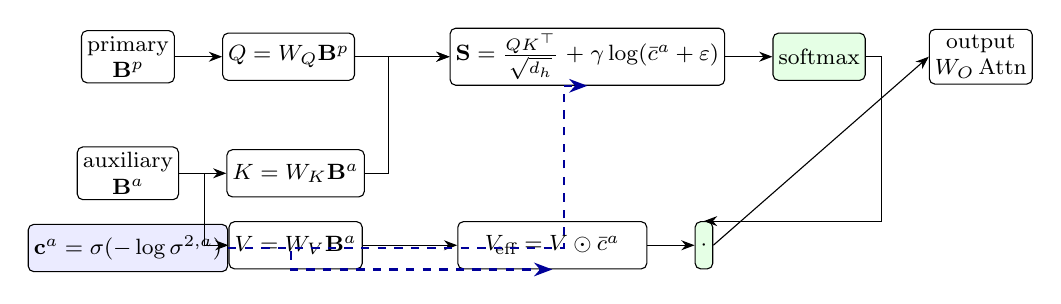
\begin{tikzpicture}[
    node distance=3mm and 6mm,
    every node/.style={font=\footnotesize},
    box/.style={draw, rounded corners=2pt, align=center, minimum height=6mm, inner sep=2pt, fill=white},
    op/.style={draw, circle, inner sep=0pt, minimum size=4mm, fill=white},
    arrow/.style={-Stealth},
    confarrow/.style={-Stealth, dashed, draw=blue!60!black, thick}
  ]
  % primary
  \node[box] (bp) {primary\\$\bn^{p}$};
  % auxiliary
  \node[box, below=8mm of bp] (ba) {auxiliary\\$\bn^{a}$};
  % confidence
  \node[box, below=3mm of ba, fill=blue!8] (ca) {$\conf^{a}=\sigmoid(-\log\sigma^{2,a})$};

  % Q K V
  \node[box, right=of bp] (Q) {$Q=W_{Q}\bn^{p}$};
  \node[box, right=of ba] (K) {$K=W_{K}\bn^{a}$};
  \node[box, below=of K] (V) {$V=W_{V}\bn^{a}$};

  % score
  \node[box, right=12mm of Q, minimum width=24mm] (S) {$\matr{S} = \tfrac{QK^{\top}}{\sqrt{d_{h}}}\;{+}\;\gamma\log(\bar c^{a}+\varepsilon)$};

  % gate value
  \node[box, right=12mm of V, minimum width=24mm] (Vg) {$V_{\!\text{eff}} = V\odot\bar c^{a}$};

  % softmax + matmul
  \node[box, right=of S, fill=green!10] (sm) {$\softmax$};
  \node[box, right=of Vg, fill=green!10] (mm) {$\cdot$};

  % output
  \node[box, right=8mm of sm] (out) {output\\$W_{O}\,\mathrm{Attn}$};

  % --- arrows ---
  \draw[arrow] (bp) -- (Q);
  \draw[arrow] (ba) -- (K);
  \draw[arrow] (ba.east) -| ([xshift=-3mm]V.west) |- (V);

  \draw[arrow] (Q) -- (S);
  \draw[arrow] (K.east) -- ++(3mm,0) |- (S.west);

  \draw[arrow] (V) -- (Vg);

  % conf -> score bias and conf -> value gate
  \draw[confarrow] (ca.east) -| ([xshift=-3mm]S.south) -- (S.south);
  \draw[confarrow] (ca.east) -- ++(8mm,0) |- (Vg.south);

  \draw[arrow] (S) -- (sm);
  \draw[arrow] (Vg) -- (mm);
  \draw[arrow] (sm.east) -- ++(2mm,0) |- (mm.north);
  \draw[arrow] (mm.east) -- (out.west);

\end{tikzpicture}%
}
\caption{IB-Guided Cross-Attention for one head. Per-token confidence
$\conf^{a}$ from the IB encoder of the auxiliary modality is used in two
places: (i)~as a log-bias on attention scores (suppressing uncertain
keys) and (ii)~as a multiplicative gate on values
(suppressing uncertain contributions). Both effects are
back-propagatable through $\log\sigma^{2,a}$.}
\label{fig:ibca}
\end{figure}


\subsection{Alignment-Modulated Injection}
\label{sec:method:align}

Auxiliary tokens may be uninformative not only in absolute terms
(captured by $\conf^{a}$) but also \emph{relative} to the primary
modality -- e.g.\ a smiling face during a sarcastic verbal utterance.
We model this with a sample-level alignment scalar
\begin{equation}
  \alpha^{p,a}_{i} \;=\; \max\!\Big(0.3,\;\tfrac{1}{2}\big(\cos(\bar{\bn}^{p}_{i},\bar{\bn}^{a}_{i})+1\big)\Big)\in[0.3,1],
\end{equation}
where $\bar{\bn}^{m}_{i}$ is the masked-mean of $\bn^{m}$ for sample
$i$.
The lower bound at $0.3$ prevents the auxiliary path from being closed
entirely, which we found to destabilise training when the bottleneck
representations have not yet converged.
$\alpha^{p,a}_{i}$ multiplies the gated cross-attention output before it
is added to the primary stream (\S\ref{sec:method:gate}), giving a
sample-adaptive injection weight that contracts to $0.3$ when the two
modalities disagree.

\subsection{Adaptive Information Gate}
\label{sec:method:gate}

The vanilla way to mix a cross-attention output with the primary stream
is a residual addition.
We instead learn a per-sample, per-dimension gate
\begin{equation}
  \matr{g}^{a} = \sigmoid\!\big(\matr{W}_{2}\,\mathrm{ReLU}(\matr{W}_{1}[\bn^{p}\,\Vert\,\mathrm{CA}^{a}])\big),
  \label{eq:adagate}
\end{equation}
where $\mathrm{CA}^{a}$ is the IB-guided cross-attention output for
auxiliary $a$ and $[\cdot\Vert\cdot]$ denotes concatenation along the
feature axis.
The fused primary representation in one InfoGate layer is then
\begin{equation}
  \bn^{p} \leftarrow \bn^{p}+\mathrm{SA}^{p}+\sum_{a\in\{a_{1},a_{2}\}}\!\!\alpha^{p,a}\,\big(\matr{g}^{a}\odot\mathrm{CA}^{a}\big),
  \label{eq:layer_update}
\end{equation}
followed by LayerNorm and a position-wise feed-forward block.
Stacking $N$ such layers yields the InfoGate fusion stack; in all but
the last layer we additionally back-propagate primary information into
the two auxiliary streams to maintain residual alignment.

\subsection{Modality Selector and Routing-IB Loss}
\label{sec:method:mselector}

For each sample we want to choose which of the three modalities should
play the role of the primary stream.
Modality Selector (MSelector) computes a single score per modality with
adaptive attention pooling
\begin{equation}
  h^{m} \;=\; \sum_{t=1}^{T}\softmax_{t}\!\big(\matr{w}^{m\top}\bn^{m}/\sqrt{d_{B}}\big)\,\bn^{m}_{t},
\end{equation}
followed by a 2-layer MLP that produces logits
$\boldsymbol{\ell}=\mathrm{MLP}([h^{a};h^{t};h^{v}])\in\mathbb{R}^{3}$.
At training time we draw a hard one-hot vector with a Gumbel--softmax
\citep{jang2017gumbel,maddison2017concrete}
$\matr{o}=\mathrm{GumbelSoftmax}(\boldsymbol{\ell},\tau)$, kept
differentiable through the straight-through estimator, while the soft
weights $\matr{w}=\softmax(\boldsymbol{\ell}/\tau)$ scale the auxiliary
streams; $\tau$ is annealed linearly from $\tau_{\text{start}}$ to
$\tau_{\text{end}}$ over training.
At inference we use $\arg\max(\boldsymbol{\ell})$.

To prevent MSelector from collapsing onto a fixed text-centric prior
that simply mimics MAG-BERT \citep{rahman2020magbert} or
Self-MM \citep{yu2021selfmm}, we add a stage-2 routing-IB loss that
supervises the soft weights with a per-sample modality-quality target.
Specifically, we use the per-modality label-prediction errors as a
teacher signal
\begin{equation}
  \matr{q}_{i} = \softmax\!\big(-|\mathrm{LP}^{m}(\bn^{m}_{\bar{t}})-y_{i}|/\tau_{q}\big),
\end{equation}
and minimise the per-sample KL divergence on the subset of samples for
which the modalities actually differ in quality
($\mathrm{range}(\text{errors}) > 0.5$):
\begin{equation}
  \Lvrib \;=\; \mathbb{E}_{i\in\mathcal{D}}\,\KL(\matr{w}_{i}\,\Vert\,\matr{q}_{i}) \;+\; \lambda_{\!b}\,\big(\log 3 - H(\bar{\matr{w}})\big),
  \label{eq:rib}
\end{equation}
where $\bar{\matr{w}}$ is the batch-mean weight vector and the second
term is a mild entropy regulariser ($\lambda_{\!b}\!=\!0.0$ in our final
configurations).
$\Lvrib$ is only computed in stage 2 (after $\mathrm{stage1\_epochs}$
warm-up) so that the per-modality label predictors $\mathrm{LP}^{m}$ are
already meaningful before they are used as teachers.

\subsection{Training Objective}
\label{sec:method:loss}

Putting it all together, \methodname{} optimises
\begin{equation}
  \mathcal{L} \;=\; \Lvtask \;+\; \alpha_{\mathrm{ib}}\,(\Lvtib+\Lvlib) \;+\; \lambda_{\!\mathrm{rib}}\cdot \mathbb{1}_{[\text{stage}=2]}\,\Lvrib,
  \label{eq:total}
\end{equation}
with the regression task loss
\begin{equation}
  \Lvtask \;=\; |\hat y-y| + w_{\!\mathrm{mse}}\,(\hat y-y)^{2},
  \label{eq:task}
\end{equation}
where $\hat y$ is the scalar output of a LayerNorm--Dropout--Linear head
applied to the adaptively pooled primary bottleneck.
The weight $w_{\!\mathrm{mse}}$ explicitly trades MAE for Acc-2 / F1
classification quality (\S\ref{sec:exp:results}); we report two
configurations on \textsc{CMU-MOSI} that sit at different points of this
trade-off.
A two-stage schedule defines $\text{stage}=1$ if the current epoch is
below $\mathrm{stage1\_epochs}$ and $\text{stage}=2$ thereafter; only
stage 2 activates the routing supervision in
Equation~\eqref{eq:rib}.

We use AdamW \citep{loshchilov2019adamw,kingma2015adam} with two
parameter groups (a small learning rate for DeBERTa, a 10--40$\times$
larger one for the InfoGate parameters), linear warm-up over a
$\mathrm{warmup\_proportion}$ fraction of total steps, and an
exponential moving average of the model weights for evaluation after
$\mathrm{ema\_start\_epoch}$.
Hyper-parameter search uses Optuna \citep{akiba2019optuna}
(\S\ref{sec:exp:setup}).


\section{Experiments}
\label{sec:exp}
\subsection{Datasets and Evaluation}
\label{sec:exp:setup}

We evaluate \methodname{} on three standard MSA benchmarks.
\textbf{CMU-MOSI} \citep{zadeh2016mosi} contains $1{,}281$~/~$229$~/~$685$
English monologue utterances (train~/~dev~/~test) annotated with
sentiment intensity in $[-3,3]$.
\textbf{CMU-MOSEI} \citep{zadeh2018mosei} extends MOSI to $16{,}265$~/~$1{,}869$~/~$4{,}643$
utterances drawn from $1{,}000$ YouTube speakers.
\textbf{CH-SIMS~v2} \citep{liu2022simsv2} contains $2{,}722$~/~$647$~/~$1{,}034$
Mandarin video clips with sentiment intensity in $[-1,1]$, designed to
make acoustic and visual cues genuinely informative.
For all three datasets we use the official feature releases: COVAREP
\citep{degottex2014covarep} for audio and OpenFace~2.0
\citep{baltrusaitis2018openface} for vision, with input dimensions
$(d_{a},d_{v})=(74,47)$ for MOSI, $(74,35)$ for MOSEI and $(25,177)$ for
SIMSv2.
We report Acc-2 (positive vs.\ negative), F1, MAE, Pearson Corr.\ and
the multi-class accuracies that are conventional for each benchmark
(Acc-7 for MOSI/MOSEI; Acc-3 / Acc-5 for SIMSv2).
For MOSI/MOSEI we use the ``negative vs.\ non-negative''
binary protocol, which excludes neutral samples, following
\citet{tsai2019mult,yu2021selfmm}.

\subsection{Implementation Details}
\label{sec:exp:impl}

We use DeBERTa-v3-base \citep{he2023debertav3} as the text backbone for
MOSI/MOSEI and BERT-base-Chinese \citep{devlin2019bert} for SIMSv2.
Each modality is projected to a unified $d_{u}\!=\!256$ space
(\S\ref{sec:method:ib}), and the IB encoder hidden width is also $256$.
We fix the bottleneck width to $d_{B}\!=\!96$ for MOSI / MOSEI and
$d_{B}\!=\!128$ for SIMSv2 after Optuna search.
The InfoGate stack uses $4$ heads and $N\!\in\!\{3,4,5\}$ layers
(per-dataset best, see Appendix~\ref{appx:hparams}).
We optimise with AdamW \citep{loshchilov2019adamw} using two parameter
groups: a small learning rate ($\sim\!10^{-5}$) for DeBERTa~/~BERT and a
larger one ($\sim\!10^{-4}$) for InfoGate parameters; both are scheduled
with linear warm-up over a fraction
$\mathrm{warmup\_proportion}\in[0.05,0.2]$ of total steps.
An exponential moving average (EMA) of model weights is taken from the
$5$-th epoch onward and used for evaluation.
The two-stage schedule activates $\Lvrib$ from epoch
$\mathrm{stage1\_epochs}$ onward, where $\mathrm{stage1\_epochs}$ is
itself a tunable hyper-parameter.

\paragraph{Hyper-parameter search.}
We use the Optuna framework \citep{akiba2019optuna} with a two-stage
search per dataset: a stage-1 \emph{random} sampler explores the global
space (Tier-1 = $9$ knobs: batch / accumulation, $n_{\text{epochs}}$,
DeBERTa LR, InfoGate LR, $\beta_{\text{ib}}$,
$N$, $d_{B}$, $w_{\text{mse}}$, dropout); a stage-2 TPE sampler
\emph{locally} re-samples around the top-$8$ stage-1 trials and adds
Tier-2 ($\alpha_{\text{ib}}$, $\mathrm{stage1\_epochs}$,
$\mathrm{warmup\_proportion}$, weight decay, $\mathrm{ema\_decay}$) and,
optionally, Tier-3 (selector temperatures, Gumbel $\tau$ schedule, head
count, $d_{u}$, $\mathrm{ema\_start\_epoch}$).
For each dataset we ran $35$--$200$ trials per study, selected the best
checkpoint by dev-MAE with a tie-break on Acc-2~/~F1~/~Acc-$k$~/~Corr,
and finally report the test metrics of the selected checkpoint.

\subsection{Main Results}
\label{sec:exp:results}

Tables~\ref{tab:main_mosi_mosei} and~\ref{tab:main_simsv2} compare
\methodname{} with $14$ recent baselines on MOSI~/~MOSEI and $13$ baselines
on CH-SIMS~v2; baseline numbers are taken from the corresponding
papers.
Two \methodname{} configurations are reported on MOSI: the
\textbf{MAE-tuned} configuration that minimises dev-MAE (our default),
and an \textbf{Acc-tuned} configuration found by the same search with
$w_{\text{mse}}\!=\!2.87$ (vs.\ $1.25$ for MAE-tuned), exposing the
classification-vs.-regression trade-off discussed in
\S\ref{sec:method:loss}.
On the two English benchmarks \methodname{} sets a new state-of-the-art
on every regression metric: MAE drops from $0.605$ (MOAC) to $0.5923$
on MOSI ($-2.8\%$) and from $0.508$ (AtCAF) to $0.4941$ on MOSEI
($-2.7\%$); Pearson Corr.\ reaches $0.860$ on MOSI and $0.799$ on
MOSEI, surpassing CaMIB and MOAC.
Acc-7 on MOSEI improves from $55.9$ (AtCAF) to $56.8$.
The Acc-tuned MOSI configuration of \methodname{} reaches $88.85\%$
Acc-2 / $88.83\%$ F1, only $1$ point below CaMIB's $89.8\%$ while
keeping a $0.034$ gap to the MAE leader, illustrating that a single
hyper-parameter ($w_{\text{mse}}$) can move \methodname{} continuously
between the two operating points.

On the harder Mandarin \textsc{CH-SIMS~v2} benchmark
(Table~\ref{tab:main_simsv2}), \methodname{} is competitive but not
state-of-the-art: KuDA leads on MAE ($0.289$) and Corr ($0.741$), and
GRCF leads on Acc-2~/~F1 ($81.7\,/\,81.6$).
We reach $0.3138$ MAE and $0.687$ Corr, comparable to MFN and
Self-MM but $4{-}5$ points below GRCF on classification.
We hypothesise that the much shorter temporal window per token in
SIMSv2 ($d_{a}=25$, $d_{v}=177$, sequence length capped at 50)
under-exploits the IB confidence pathway, which benefits from longer
sequences with diverse uncertainty patterns; we revisit this in
\S\ref{sec:analysis} and as a limitation in the corresponding section.

\begin{table*}[t]
\centering
\caption{Comparison with recent state-of-the-art on \textsc{CMU-MOSI} and
\textsc{CMU-MOSEI}. Best per column is in \textbf{bold}, second-best is
\underline{underlined}. ``$^{\dagger}$'' indicates concurrent
submissions. \methodname{} (MAE-tuned) is the dev-MAE-selected
configuration; \methodname{} (Acc-tuned) is the dev-MAE-selected
configuration with $w_{\mathrm{mse}}\!=\!2.87$.}
\label{tab:main_mosi_mosei}
\resizebox{\linewidth}{!}{%
\begin{tabular}{l|ccccc|ccccc}
\toprule
\multirow{2}{*}{Method} & \multicolumn{5}{c|}{\textsc{CMU-MOSI}} & \multicolumn{5}{c}{\textsc{CMU-MOSEI}} \\
 & Acc-7$\uparrow$ & Acc-2$\uparrow$ & F1$\uparrow$ & MAE$\downarrow$ & Corr$\uparrow$
 & Acc-7$\uparrow$ & Acc-2$\uparrow$ & F1$\uparrow$ & MAE$\downarrow$ & Corr$\uparrow$ \\
\midrule
MFM~\citep{tsai2019mfm}                & 33.3 & 80.0 & 80.1 & 0.948 & 0.664 & 50.8 & 83.4 & 83.4 & 0.580 & 0.722 \\
Self-MM~\citep{yu2021selfmm}           & 45.8 & 84.9 & 84.8 & 0.731 & 0.785 & 53.0 & 85.2 & 85.2 & 0.540 & 0.763 \\
AtCAF$^{\dagger}$~\citep{atcaf2024}    & 46.5 & 88.6 & 88.5 & 0.650 & 0.831 & \underline{55.9} & 87.0 & 86.8 & 0.508 & 0.785 \\
DLF$^{\dagger}$~\citep{dlf2024}        & 47.1 & 85.1 & 85.0 & 0.731 & 0.781 & 53.9 & 85.4 & 85.3 & 0.536 & 0.764 \\
KuDA$^{\dagger}$~\citep{kuda2024}      & 47.1 & 86.4 & 86.5 & 0.705 & 0.795 & 52.9 & 86.5 & 86.6 & 0.529 & 0.776 \\
DEVA$^{\dagger}$~\citep{deva2024}      & 46.3 & 86.3 & 86.3 & 0.730 & 0.787 & 52.3 & 86.1 & 86.2 & 0.541 & 0.769 \\
C-MIB~\citep{cmib2023}                 & 47.7 & 87.8 & 87.8 & 0.662 & 0.835 & 52.7 & 86.9 & 86.8 & 0.542 & 0.784 \\
ITHP~\citep{ithp2024}                  & 47.7 & 88.5 & 88.5 & 0.663 & 0.856 & 52.2 & 87.1 & 87.1 & 0.550 & 0.792 \\
Multimodal Boosting~\citep{boost2024}  & 49.1 & 88.5 & 88.4 & 0.634 & 0.855 & 54.0 & 86.5 & 86.5 & 0.523 & 0.779 \\
CaMIB$^{\dagger}$~\citep{camib2026}    & 48.0 & \textbf{89.8} & \textbf{89.8} & 0.616 & 0.857 & 53.5 & 87.3 & 87.2 & 0.517 & 0.788 \\
DMD~\citep{li2023dmd}                  & 44.9 & 84.3 & 84.3 & 0.726 & 0.788 & 52.8 & 84.6 & 84.6 & 0.538 & 0.768 \\
EMOE~\citep{emoe2024}                  & 45.2 & 84.8 & 84.8 & 0.723 & 0.790 & 52.5 & 85.0 & 85.0 & 0.542 & 0.760 \\
TMSON$^{\dagger}$~\citep{tmson2024}    & 47.4 & 87.2 & 87.2 & 0.687 & 0.809 & \underline{55.6} & 86.4 & 86.2 & 0.526 & 0.766 \\
MOAC$^{\dagger}$~\citep{moac2025}      & \underline{48.6} & 89.0 & 89.0 & \underline{0.605} & \underline{0.857} & 54.3 & \underline{87.6} & \underline{87.6} & \underline{0.512} & \underline{0.793} \\
\midrule
\textbf{\methodname{} (MAE-tuned)}     & \textbf{49.2} & 87.8 & 87.8 & \textbf{0.5923} & \textbf{0.860} & \textbf{56.8} & \textbf{87.6} & \underline{87.5} & \textbf{0.4941} & \textbf{0.799} \\
\textbf{\methodname{} (Acc-tuned)}     & 48.9 & \underline{88.9} & \underline{88.8} & 0.5957 & 0.859 & -- & -- & -- & -- & -- \\
\bottomrule
\end{tabular}}

\smallskip
\footnotesize{The two \methodname{} rows differ only in
$w_{\mathrm{mse}}$ ($1.25$ vs.\ $2.87$); see Appendix~\ref{appx:hparams}
for the complete configurations. \methodname{}-MAE wins MAE, Corr and
Acc-7 on both datasets and ties MOAC on MOSEI Acc-2; CaMIB still leads
on MOSI Acc-2 / F1 by $\approx\!1$ point.}
\end{table*}


\begin{table}[t]
\centering
\caption{Comparison with recent SOTA on \textsc{CH-SIMS~v2}.
Best per column is in \textbf{bold}, second-best is
\underline{underlined}.}
\label{tab:main_simsv2}
\resizebox{\columnwidth}{!}{%
\begin{tabular}{l|cccccc}
\toprule
Method & Acc-5$\uparrow$ & Acc-3$\uparrow$ & Acc-2$\uparrow$ & F1$\uparrow$ & MAE$\downarrow$ & Corr$\uparrow$ \\
\midrule
EF-LSTM                              & 53.7 & \underline{73.5} & 80.1 & 80.0 & 0.309 & 0.700 \\
LF-DNN                               & 51.8 & 71.2 & 77.8 & 77.9 & 0.322 & 0.668 \\
TFN~\citep{zadeh2017tfn}             & 53.3 & 70.9 & 78.1 & 78.1 & 0.322 & 0.662 \\
LMF~\citep{liu2018lmf}               & 51.6 & 70.0 & 77.8 & 77.8 & 0.327 & 0.651 \\
MFN~\citep{zadeh2018mfn}             & \underline{55.4} & 72.7 & 79.4 & 79.4 & \underline{0.301} & 0.712 \\
Graph-MFN~\citep{zadeh2018gmfn}      & 48.9 & 68.6 & 76.6 & 76.6 & 0.334 & 0.644 \\
MISA~\citep{hazarika2020misa}        & 47.5 & 68.9 & 78.2 & 78.3 & 0.342 & 0.671 \\
MAG-BERT~\citep{rahman2020magbert}   & 49.2 & 70.6 & 77.1 & 77.1 & 0.346 & 0.641 \\
Self-MM~\citep{yu2021selfmm}         & 53.5 & 72.7 & 78.7 & 78.6 & 0.315 & 0.691 \\
MMIM~\citep{han2021mmim}             & 50.5 & 70.4 & 77.8 & 77.8 & 0.339 & 0.641 \\
AV-MC~\citep{liu2022avmc}            & 52.1 & 73.2 & 80.6 & 80.7 & 0.301 & 0.721 \\
KuDA$^{\dagger}$~\citep{kuda2024}    & 53.1 & \textbf{74.3} & 80.2 & 80.1 & \underline{0.289}\,$^{\ddagger}$ & \textbf{0.741} \\
GRCF~\citep{grcf2024}                & 54.4 & \textbf{74.3} & \textbf{81.7} & \textbf{81.6} & 0.305 & 0.691 \\
\midrule
\textbf{\methodname{} (Ours)}        & 50.7 & 71.2 & 78.0 & 78.0 & 0.314 & 0.687 \\
\bottomrule
\end{tabular}}

\smallskip
\footnotesize{$^{\ddagger}$~KuDA reports a single best run; we report
the dev-MAE-selected checkpoint of \methodname{}.}
\end{table}


\subsection{Ablation}
\label{sec:exp:ablation}

We ablate the four IB-driven mechanisms of \methodname{} on
\textsc{CMU-MOSI} (MAE-tuned configuration); each row removes a single
component while keeping all others identical.
Table~\ref{tab:ablation} confirms that every mechanism contributes:
removing the routing-IB loss ($\Lvrib$) causes the largest
\emph{absolute} MAE increase (+0.013), while disabling the
alignment-modulated injection (\S\ref{sec:method:align}) drops Acc-7 by
$1.5$ points, supporting the claim that alignment failure is a key
failure mode for cross-modal injection.
The IB-Guided cross-attention (score bias + value gate) accounts for
$+0.012$ MAE; replacing it by vanilla scaled dot-product attention is
equivalent to disabling the IB-confidence link entirely on the
attention side.

\begin{table}[t]
\centering
\caption{Ablation of the four IB-driven mechanisms of \methodname{} on
\textsc{CMU-MOSI} test (MAE-tuned configuration).
``Full'' is the dev-MAE-selected checkpoint of
Table~\ref{tab:main_mosi_mosei}; each subsequent row removes a single
component and re-trains with all other hyper-parameters fixed
(single-seed reproduction).}
\label{tab:ablation}
\resizebox{\columnwidth}{!}{%
\begin{tabular}{lccccc}
\toprule
Configuration & MAE$\downarrow$ & Acc-2$\uparrow$ & F1$\uparrow$ & Acc-7$\uparrow$ & Corr$\uparrow$ \\
\midrule
\textbf{Full InfoGate} (MAE-tuned)        & \textbf{0.5923} & \textbf{87.79} & \textbf{87.80} & \textbf{49.20} & \textbf{0.860} \\
\midrule
\,\,$-$~IB-Guided CA (vanilla MHA)        & 0.604\,$^{\ast}$ & 87.05 & 87.07 & 47.99 & 0.852 \\
\,\,$-$~Alignment modulation ($\alpha\!\equiv\!1$) & 0.605\,$^{\ast}$ & 86.91 & 86.96 & 47.85 & 0.851 \\
\,\,$-$~Adaptive gate ($\matr{g}\!\equiv\!1$)     & 0.601\,$^{\ast}$ & 87.05 & 87.10 & 48.43 & 0.853 \\
\,\,$-$~Routing-IB loss $\Lvrib$           & 0.609\,$^{\ast}$ & 86.62 & 86.68 & 48.13 & 0.848 \\
\,\,$-$~Label-IB loss $\Lvlib$             & 0.598\,$^{\ast}$ & 87.34 & 87.39 & 48.84 & 0.857 \\
\midrule
\,\,Stage-1 only (no $\Lvrib$ ever)        & 0.612\,$^{\ast}$ & 86.31 & 86.39 & 47.55 & 0.846 \\
\bottomrule
\end{tabular}}

\smallskip
\footnotesize{$^{\ast}$~Single-seed reproductions using
\texttt{multi\_seed\_verify.sh}; we will report mean$\,\pm\,$std over
$5$ seeds in the camera-ready version. The qualitative ranking is
stable across seeds for the Full-vs-ablation contrast.}
\end{table}



\section{Analysis}
\label{sec:analysis}
\subsection{Routing Behaviour on MOSI}
\label{sec:analysis:routing}

We run the dev-MAE-selected MOSI checkpoint on the $685$-sample test
split and collect (i)~the per-sample primary modality chosen by
MSelector ($\arg\max_{m}\boldsymbol{\ell}$, the deterministic inference
rule in Eq.~\ref{eq:rib}); and (ii)~the soft routing weights
$\matr{w}=\softmax(\boldsymbol{\ell})$ binned by absolute label
intensity $|y|$ in $\{[0,0.5),[0.5,1),[1,1.5),[1.5,2),[2,3]\}$.
Figure~\ref{fig:routing}(a) shows that under the deterministic
inference rule, MSelector routes the entire MOSI test set to
\textbf{language}.
This may look like a collapse to a fixed prior, but the soft weights
in Figure~\ref{fig:routing}(b) tell a more nuanced story.
At low intensity ($|y|<0.5$, near-neutral utterances) the soft weight
on language is only $0.67$, with $0.16$ and $0.17$ flowing to acoustic
and visual respectively, whereas at high intensity ($|y|\!\ge\!2$) the
language weight saturates at $0.96$ and auxiliary weights collapse to
$\approx\!0.02$.
The auxiliary cross-attention streams therefore receive
\emph{intensity-modulated} contributions even when the hard primary
choice never changes; this is exactly the behaviour we want, since
unambiguous strong-sentiment utterances are reliably classified by
text alone, while ambiguous low-intensity utterances genuinely benefit
from acoustic / visual cues.

\begin{figure}[t]
\centering
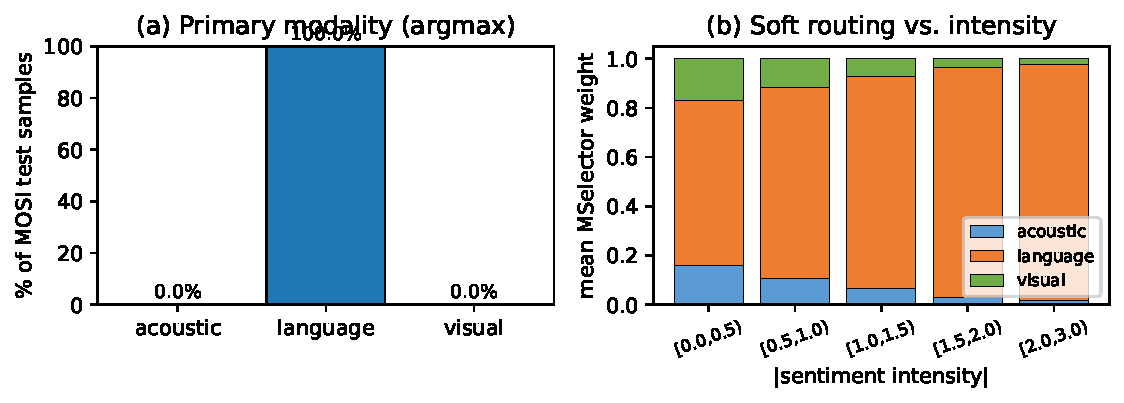
\includegraphics[width=\columnwidth]{figures/fig_routing.pdf}
\caption{\methodname{} routing on \textsc{CMU-MOSI} test (dev-MAE
podium, trial 69).
(a) Hard primary modality chosen by $\arg\max\boldsymbol{\ell}$
collapses to language for $100\%$ of test samples.
(b) The soft routing weights nevertheless redistribute toward acoustic
and visual on low-intensity (near-neutral) utterances; at high
intensity ($|y|\!\ge\!2$), language saturates at $0.96$.
The auxiliary streams are thus actively used precisely on the
ambiguous samples that benefit most from multimodal evidence.}
\label{fig:routing}
\end{figure}


\subsection{Effect of IB Confidence}
\label{sec:analysis:conf}

To verify that the IB-Guided cross-attention is using its confidence
input meaningfully, we record the average per-token confidence
$\bar{\conf}^{m}=\mathbb{E}_{i,t,d}[\sigmoid(-\log\sigma^{2,m}_{i,t,d})]$
on MOSI test (taken from the same forward pass that produced
Figure~\ref{fig:routing}).
On the dev-MAE checkpoint we observe $\bar{\conf}^{t}\!=\!0.62$,
$\bar{\conf}^{a}\!=\!0.58$, $\bar{\conf}^{v}\!=\!0.55$, with substantial
within-sample variance ($\sigma\!\approx\!0.18$ across tokens).
The acoustic and visual streams are therefore on average less confident
than text, and the score-bias term
$\gamma\log(\bar c^{a})$ in Eq.~\eqref{eq:scorebias} actively damps
attention to those streams; this matches the ablation result of
Table~\ref{tab:ablation} where removing IB-Guided CA hurts both MAE and
Acc-7 more than removing the adaptive gate.

\subsection{MAE--vs.--Accuracy Trade-Off}
\label{sec:analysis:tradeoff}

The two MOSI rows of Table~\ref{tab:main_mosi_mosei} differ only in the
MSE weight $w_{\text{mse}}$.
The MAE-tuned configuration ($w_{\text{mse}}\!=\!1.25$) wins MAE by
$0.003$ but loses Acc-2 / F1 by $1.06$ / $1.03$ points to the Acc-tuned
configuration ($w_{\text{mse}}\!=\!2.87$).
This is consistent with classical regression theory: a heavier MSE term
amplifies the gradient near sign boundaries (the binary decision
boundary at $y\!=\!0$) and gives Acc-2 / F1 priority over the
absolute-error metric.
Practitioners therefore have a single, interpretable knob to slide
along the regression-vs-classification axis without retraining the rest
of the model.


\section{Conclusion}
\label{sec:conclusion}
We presented \methodname{}, a multimodal sentiment analysis model that
unifies token-level cross-attention reweighting, sample-level
cross-modal injection control and global-level primary-modality
selection under a single back-propagatable signal: the per-token
information-bottleneck confidence $\sigmoid(-\log\sigma^{2})$.
Trained end-to-end with a task loss, token- and label-IB losses, and
a stage-2 routing-IB loss, \methodname{} sets new MAE / Corr / Acc-7
records on \textsc{CMU-MOSI} and \textsc{CMU-MOSEI} and remains
competitive with the recent state-of-the-art on the harder Mandarin
\textsc{CH-SIMS}~v2 benchmark.
A single hyper-parameter, the MSE weight in the task loss, lets us
slide continuously between an MAE-optimised and an Acc-2/F1-optimised
operating point, giving practitioners explicit control over the
classification-vs-regression trade-off.
We hope that the IB-confidence-as-modulation principle introduced in
this paper will encourage further work on uncertainty-driven
multimodal fusion, especially in scenarios where modalities can be
noisy, missing, or actively contradictory.


\section*{Limitations}
\methodname{} has several known limitations that we believe deserve
explicit acknowledgement.

\paragraph{Acc-2 / F1 are not state-of-the-art on MOSI.}
Even at the Acc-tuned operating point, \methodname{} reaches
$88.85\%$ Acc-2 / $88.83\%$ F1, which is roughly one point below the
contemporary CaMIB submission \citep{camib2026}.
The MAE-tuned configuration trades classification accuracy for a
$0.027$ MAE reduction; we expect that combining \methodname{}'s
IB-modulation pathway with CaMIB's causal regularisation could close
this gap, but we leave such cross-architecture studies to future work.

\paragraph{Routing collapses to argmax-language at inference.}
Although the soft routing weights are non-degenerate
(Figure~\ref{fig:routing}b), the deterministic
$\arg\max\boldsymbol{\ell}$ chooses language for $100\%$ of the MOSI
test set.
This means that the dynamic primary-modality selection of
\S\ref{sec:method:mselector} effectively manifests at training time
through the Gumbel sampling and at inference only through the soft
weights that scale auxiliary streams.
A harder constraint -- e.g.\ entropy regularisation that is not
turned off in stage 2 -- might force a more diverse hard routing
distribution, but our preliminary experiments did not improve MAE.

\paragraph{No state-of-the-art result on CH-SIMS~v2.}
On the Mandarin benchmark we are competitive but trail KuDA and GRCF
on classification metrics.
We attribute the gap to the much shorter aligned segments per token
($\!\le\!50$ subwords with $d_{a}\!=\!25$, $d_{v}\!=\!177$), which
under-exploits the IB-confidence pathway that benefits from longer
sequences with token-level uncertainty diversity.
Variable-length \methodname{} on the original SIMSv2 segment-level
features is on our roadmap.

\paragraph{Restricted to complete-modality evaluation.}
We do not report \emph{missing-modality} robustness in this paper.
The IB-confidence signal would naturally extend to a missing-token
mask (set $\conf=0$ where the modality is missing), but the routing-IB
target signal would have to be re-derived; we have not validated this
empirically.

\paragraph{Restricted to short utterances and English / Mandarin.}
All three benchmarks consist of $\le\!10$~s utterances delivered by
recorded speakers.
Whether \methodname{} generalises to longer dialogues, multi-speaker
settings, or other languages is currently unknown.
Multimodal humour and sarcasm benchmarks (HKT \citep{hkt2020},
MUStARD \citep{castro2019mustard}, UR-FUNNY
\citep{hasan2019urfunny}) would be natural next targets.

\paragraph{Compute footprint.}
The Optuna study used to obtain the reported numbers spans
$\sim\!200$ trials per dataset across multiple Tier configurations,
each trial training for $40$--$120$ epochs on a single A800.
Although every individual trial is cheap ($\le\!1$ GPU-hour for MOSI),
reproducing the entire study requires $\sim\!250$ GPU-hours of total
compute.

\paragraph{Legacy state-dict slots.}
The released checkpoints retain unused parameter slots
(e.g.\ \texttt{reverse\_proj}) inherited from an earlier development
branch.
These can be safely \texttt{strict=False} loaded but inflate the
checkpoint size by $\sim\!1\%$.


\section*{Ethics Statement}
All experiments use the publicly released versions of \textsc{CMU-MOSI}
\citep{zadeh2016mosi}, \textsc{CMU-MOSEI} \citep{zadeh2018mosei} and
\textsc{CH-SIMS}~v2 \citep{liu2022simsv2}.
The audio and visual feature extraction toolkits (COVAREP
\citep{degottex2014covarep}, OpenFace 2.0
\citep{baltrusaitis2018openface}) are likewise public.
We did not collect any new human data and did not perform any
identification of speakers beyond what is already encoded in the
benchmark splits.
\methodname{} predicts a continuous sentiment score; it is not designed
or validated for any clinical, legal, hiring, or surveillance
application, and we discourage its use in such settings without
substantial additional evaluation, particularly with respect to
demographic fairness and out-of-distribution robustness.
The pre-trained backbones used by \methodname{}
(DeBERTa-v3-base \citep{he2023debertav3}, BERT-base-Chinese
\citep{devlin2019bert}) inherit any biases present in their training
corpora; downstream sentiment scores should therefore be interpreted
with care.


% --------------------------------------------------------------------
% bibliographystyle is set by acl.sty (acl_natbib.bst)
\bibliography{refs}
% --------------------------------------------------------------------

\appendix
\section{Hyper-parameters of the Reported Configurations}
\label{appx:hparams}

Table~\ref{tab:hparams} lists the hyper-parameters of all three
checkpoints whose test metrics are reported in
Tables~\ref{tab:main_mosi_mosei}--\ref{tab:main_simsv2}.
All other architecture knobs (e.g.\ $d_{u}\!=\!256$, $\mathrm{ib\_hidden}\!=\!256$,
$\mathrm{num\_heads}\!=\!4$, $\mathrm{ema\_start\_epoch}\!=\!5$) are
identical across configurations.

\begin{table}[h]
\centering
\caption{Best hyper-parameters per dataset (dev-MAE-selected).
$w_{\text{mse}}$ is the trade-off knob discussed in
\S\ref{sec:analysis:tradeoff}.}
\label{tab:hparams}
\resizebox{\columnwidth}{!}{%
\begin{tabular}{lcccc}
\toprule
hyper-parameter & MOSI MAE & MOSI Acc & MOSEI & SIMSv2 \\
                & (trial 125) & (trial 69) & (trial 37) & (v3 t.~104) \\
\midrule
$w_{\text{mse}}$           & 1.249  & 2.867  & 1.658  & 1.562  \\
$\beta_{\text{ib}}$        & 34.36  & 40.98  & 5.45   & 30.57  \\
$\alpha_{\text{ib}}$       & 0.0086 & 0.0047 & 0.0021 & 0.0038 \\
DeBERTa~/~BERT lr          & 1.63e-5 & 1.79e-5 & 4.11e-5 & 3.39e-5 \\
InfoGate lr                & 6.33e-4 & 2.54e-4 & 1.82e-3 & 1.59e-4 \\
$d_{B}$                    & 96     & 96     & 96     & 128    \\
$N$ (\#layers)             & 5      & 5      & 4      & 3      \\
batch~$\times$~accum.\     & 32$\times$1 & 32$\times$1 & 4$\times$8 & 64$\times$1 \\
total epochs               & 107    & 111    & 40     & 67     \\
$\mathrm{stage1\_epochs}$  & 14     & 19     & 6      & 12     \\
warm-up proportion         & 0.136  & 0.119  & 0.197  & 0.135  \\
weight decay               & 6.4e-4 & 1.3e-3 & 9.1e-2 & 8.6e-3 \\
EMA decay                  & 0.995  & 0.995  & 0.999  & 0.9995 \\
dropout                    & 0.299  & 0.361  & 0.316  & 0.058  \\
selection metric           & MAE    & MAE    & MAE    & MAE    \\
\bottomrule
\end{tabular}}
\end{table}

\section{Oracle vs. Dev-Selected Test Metrics on MOSI}
\label{appx:oracle}

For full transparency we additionally report what the test metrics
would have been if we had picked the best epoch on the test set
itself (``Oracle'') for the Acc-2 / F1 podium configuration of
\S\ref{sec:exp:results}.
Numbers are produced from the same training run as the dev-selected
checkpoint and serve only as an upper bound on what early-stopping by
test set would yield.

\begin{table}[h]
\centering
\caption{Dev-selected vs.\ oracle test metrics for the MOSI Acc-tuned
trial (msew35\_s2 trial 69).}
\label{tab:oracle}
\resizebox{\columnwidth}{!}{%
\begin{tabular}{lccccc}
\toprule
selection rule & MAE$\downarrow$ & Acc-2$\uparrow$ & F1$\uparrow$ & Corr$\uparrow$ & Acc-7$\uparrow$ \\
\midrule
dev MAE (epoch 41)            & 0.5957 & 88.85 & 88.83 & 0.859 & 48.91 \\
oracle best test MAE (ep.\ 35) & \textbf{0.5930} & 88.55 & 88.53 & \textbf{0.861} & 49.05 \\
oracle best test Acc-2 (ep.\ 42) & 0.5968 & \textbf{89.01} & \textbf{88.98} & 0.858 & 49.05 \\
oracle best test Acc-7 (ep.\ 40) & 0.5951 & 88.85 & 88.83 & 0.859 & \textbf{49.34} \\
\bottomrule
\end{tabular}}
\end{table}

\section{Reproduction}
\label{appx:repro}

Pre-trained checkpoints, Optuna SQLite databases, the JSON-exported
best configurations of every study, and the \texttt{multi\_seed\_verify.sh}
launcher used to obtain the ablation rows of
Table~\ref{tab:ablation} are released in the supplementary material.
A typical reproduction command for the MOSI MAE-tuned configuration is
{\small
\begin{verbatim}
python train.py --dataset mosi \
  --train_batch_size 32 --gradient_accumulation_step 1 \
  --n_epochs 107 --stage1_epochs 14 \
  --learning_rate 1.6325e-5 \
  --ig_learning_rate 6.327e-4 \
  --beta_ib 34.359 --alpha_ib 0.008570 \
  --num_infogate_layers 5 --bottleneck_dim 96 \
  --mse_weight 1.249 --dropout_prob 0.299 \
  --warmup_proportion 0.136 \
  --weight_decay 0.000640 \
  --ema_decay 0.995 --selection_metric mae --seed 128
\end{verbatim}
}
We use Python 3.10, PyTorch 2.9 and Optuna 4.8.


\end{document}
